
\documentclass{beamer}


%load any additional packages

\usepackage[UKenglish]{babel}
\usepackage[utf8]{inputenc} % so we can input characters with accents (e.g. ő)

\usepackage{statsbeamer}

\usepackage{graphicx} % ease graphics management
\graphicspath{{images/}} % define folder with images
\usefonttheme{serif} % change font to allow \textbf{}
\usepackage{charter} % Nicer fonts

\usepackage{amsmath,amsthm,amssymb} % for math equations

\usepackage{natbib} % richer citation
\usepackage{breakcites} % avoid overfull hbox for long cites


%% Information (author, title, etc.) %%
%\usetheme{Frankfurt}

\definecolor{mygrey}{RGB}{248, 248, 248}
\setbeamercolor{sidebar}{bg=mygrey}

\title[Lecture]{% short title for footer
    Public Opinion\\ \& \\Political Engagement
    \vspace{0.5cm}
}

\author{ Clemens Jarnach }
\institute{
        \textit{Department of Sociology}\\
        \textit{University of Oxford} \\
        \vspace{0.5cm}
        \textit{clemens.jarnach@gtc.ox.ac.uk \\ 
        \href{https://clemensjarnach.github.io}{https://clemensjarnach.github.io}}
}
\date[Venue and Date]{% short date for footer
    Oxford, 4 Aug 2023
}

% Customize the footline template to include the author's name
\setbeamertemplate{footline}{
  \begin{beamercolorbox}[sep=1em,ht=2.5ex,dp=1.125ex,leftskip=.3cm,rightskip=.3cm]{author in head/foot}
    \insertshortauthor\hfill\insertframenumber/\inserttotalframenumber
  \end{beamercolorbox}
}


%% Content of slides %%
%%%%%%%%%%%%%%%%%%%%
\begin{document}
%%%%%%%%%%%%%%%%%%%%



% Title slide %
{
    \setbeamertemplate{footline}{}
    \setbeamertemplate{headline}{}
    \setbeamercolor{background canvas}{bg=oxfordblue}

   % Temporarily redefine sidebar template for title slide
    %\setbeamertemplate{sidebar left}{}

    \maketitle

    % Restore the original sidebar template
    %\setbeamertemplate{sidebar left}[default]

}

%----------------------------%
% Contents slide
\begin{frame}{Outline}
\tableofcontents
\end{frame}
%----------------------------%

%now include the slides
%\setbeamercovered{transparent} % is used in a Beamer presentation to make covered (hidden) content transparent, rather than completely invisible, when using commands like \pause or \onslide.
%----------------------------%







% PUBLIC OPINION %%%%%%%%%%%%%%%%%%%%%%%%%%%%%%%%%%%%%%%%%%%%%%%%%
\section{Public Opinion}


\begin{frame}[plain]{Imagine there is an important election today}
\begin{itemize}
    \item How many of you would be confident in listing some of the most important political issues discussed in government right now?

    \item How well do you think your parents would do if I asked them the same question?

    \item How about people in your neighbourhood? 

    \item How about people in your state? 

    \item How about the general public? 

    \item How much does the public know about current and political affairs?
\end{itemize}
\end{frame}



\begin{frame}{What is Public Opinion?}
\begin{itemize}
    \item  Public opinion is how society collectively views political and current affairs, policy issues and political leaders. 
    \item Public opinion has a significant but somewhat unpredictable impact on politicians, politics and policy.
    \item  Public opinion matters! - at least for democratic systems
\end{itemize}
\end{frame}

%----------------------------%

\begin{frame}{Key Questions}
\begin{itemize}
    \item Do people have an opinion?
    \item Is there a collective opinion on political matters? And if so, how many?
    \item What if people don't know what they want?\\ Either due to ignorance, lack of interest, or indecisiveness.
    \item Can people express their opinion?
    \item How do people express their opinion?
    \item Does / How does / Should - the government respond to public opinions?
\end{itemize}
\end{frame}

%----------------------------%

\begin{frame}{Allocating Power}
\begin{itemize}
    \item Long lasting history of political leaders, scholars, etc being sceptical of the people's ability to make decisions on political matters (e.g. Socrates and Plato)
\end{itemize}
\end{frame}

%----------------------------%

\begin{frame}{Allocating Power}
\begin{block}{Walter Lippman}
in "Public Opinion" (1922), Walter Lippman suggests that the public's limited access to complex information might hinder their ability to make sound political judgments.
\end{block}

\begin{block}{ Joseph Schumpeter }
in "Capitalism, Socialism and Democracy" (1942) argues that the public's role in decision-making is largely reduced to choosing between competing elites, rather than direct involvement in policy formulation.
\end{block}
\end{frame}

%----------------------------%

\begin{frame}{Plato’s Ship of State (Plato, 1982)}
Imagine the governance of a state as the command of a ship.
Question: who is fit to be captain of the ship? and thus command the ship?
\begin{itemize}
    \item People = strong but near-sighted shipowner, who lack knowledge of seafaring and navigation
    \item Politicians and representatives = a group of arguing sailors, fighting for the title of captain, but also completely lacking knowledge of navigation
    \item Philosopher-king = navigator, stargazer, true captain
\end{itemize}
\end{frame}

\begin{frame}{Plato’s Ship of State (Plato, 1982)}
\begin{itemize}
    \item Is it irresponsible to let people vote without prior knowledge and training?
\end{itemize}

\end{frame}

%----------------------------%

\begin{frame}{America –  ratification of Constitution (1787-1788)}
\begin{block}{Federalists}
Strict supporters of the Constitution and a stronger national republic
\end{block}

\begin{block}{Anti-Federalists}
Those in favour of small, localised government
\end{block}

\end{frame}



\begin{frame}{Allocating Power}
The key issue is the distribution of power — to political leaders or to the people.
\begin{itemize}
    \item If the majority of people are ignorant or unable to be fully trusted with the work of governing — Strong national republic seems better (Federalists)
    \item To protect liberty and freedom of the people, smaller localised governments are better with more participation of the masses.  (Anti-Federalist)
\end{itemize}

\end{frame}




\begin{frame}{Which argument seems justified? }
\begin{itemize}
    \item Can we ask every citizen to decide on every political decision?
    \item Do citizens have the time,  money, and knowledge to make such decisions?
    \item Which decisions should be left to citizens? What kind of decisions should be made by the "experts"?
    \item Should some people get more votes than others?
    \item Who should get more votes than others?
    \item Is electing a representative just handing over your votes to that person? how is that different from giving unequal numbers of votes to people?
\end{itemize}
\end{frame}

\begin{frame}{}
These are questions we will return to at the end of this lecture...
\end{frame}


% Attention, Knowledge, Ignorance  %%%%%%%%%%%%%%%%%%%%%%%%%%%%%%%%%%%%%%%%%%%%%%%%%

\section{Interest, Knowledge, Ignorance}

\begin{frame}{Attention, Knowledge, Ignorance}
\begin{block}{Public sphere (Habermas, 1989) }
 Public sphere is an accessible social space open to public debate, where general concerns and opinions are the subject of discussion and exchange.
 \end{block}
\end{frame}

\begin{frame}{Where does Public Opinion come from?}
\end{frame}

\begin{frame}{Where does Public Opinion come from?}
    \begin{itemize}
        \item Social Network 
        \item Mass Media 
        \item Public figures (politicians, influencers) 
        \item Education 
        \item Socialisation
        \item Social/Cultural/Political Identity 
        \item Economy 
        \item Cognition 
        \itme Emotions 
        \item Current Affairs 
        \item Political Issues 
        \item etc. 
    \end{itemize} 
\end{frame}







% RESEARCH %%%%%%%%%%%%%%%%%%%%%%%%%%%%%%%%%%%%%%%%%%%%%%%%%
\section{Mass Media}

\begin{frame}{Mass Media}
\begin{itemize}
    \item Media landscape is changing, with Online media rising 
    \item Internet facilitates a high-choice media environment (Van Aelst et al., 2017)
    \item Some academics express worry regarding the rising ideological segregation among the public, attributed to novel technological shifts in the consumption of online media (Anderson, 2006; Adamic and Glance, 2005; Bozdag and Hoven, 2015; Conover et al., 2011; Sunstein, 2007).
\end{itemize}
\end{frame}

\begin{frame}{Sources of News in the UK}
    \begin{figure}
        \centering
        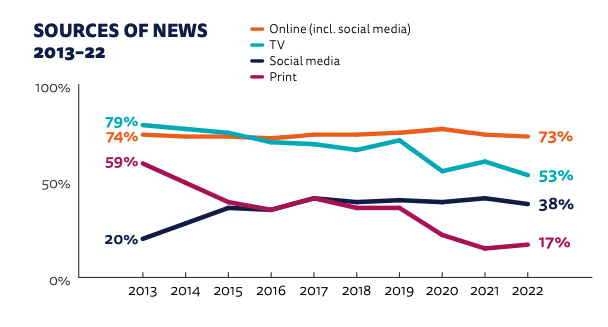
\includegraphics[width=10cm]{Reuters_Digital_News_Report_2022-UK02}
        \caption{Newman et al., 2017}
        \label{fig:1}
    \end{figure}
\end{frame}


\begin{frame}{Sources of News in the US}
    \begin{figure}
        \centering
        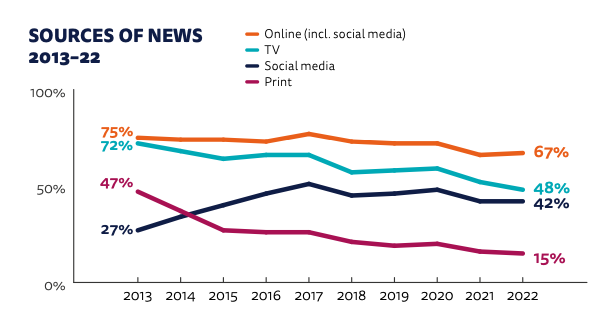
\includegraphics[width=10cm]{Reuters_Digital_News_Report_2022-USA01}
        \caption{Newman et al., 2017}
        \label{fig:my_label}
    \end{figure}
\end{frame}


\begin{frame}{Trust in News in UK}
    \begin{figure}
        \centering
        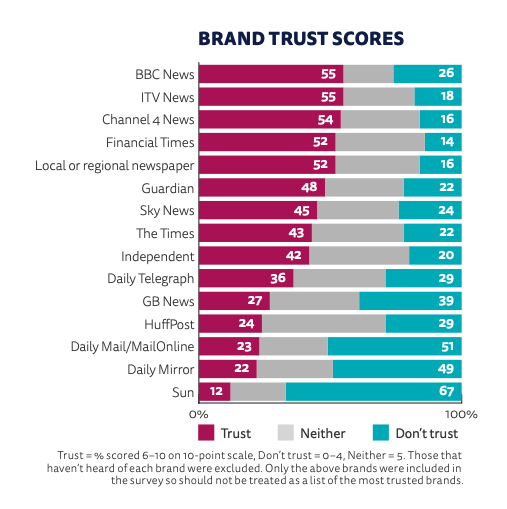
\includegraphics[width=7cm]{Reuters_Digital_News_Report_2022-UK01}
        \caption{Newman et al., 2017}
        \label{fig:my_label}
    \end{figure}
\end{frame}

\begin{frame}{Trust in News in US}
    \begin{figure}
        \centering
        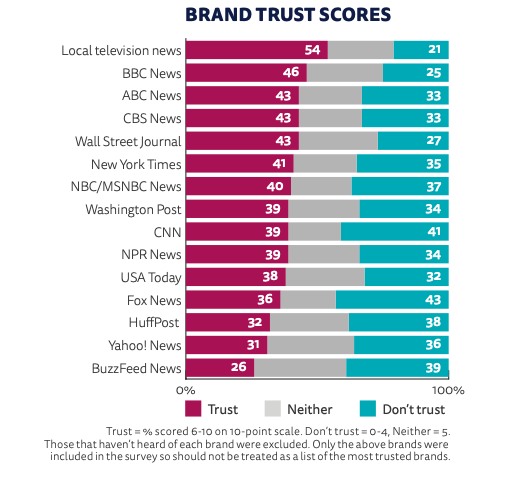
\includegraphics[width=7cm]{Reuters_Digital_News_Report_2022-UUSA-02}
        \caption{Newman et al., 2017}
        \label{fig:my_label}
    \end{figure}
\end{frame}

\begin{frame}{Trust in News in US}
    \begin{figure}
        \centering
        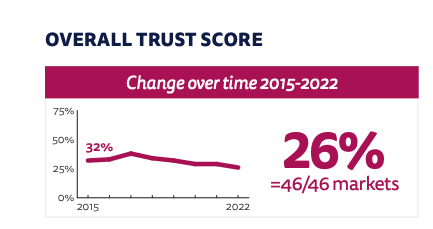
\includegraphics[width=8cm]{Reuters_Digital_News_Report_2022-UUSA-03}
        \caption{Newman et al., 2017}
        \label{fig:my_label}
    \end{figure}
\end{frame}


\begin{frame}{Media Consumption and Age in UK}
    \begin{figure}
        \centering
        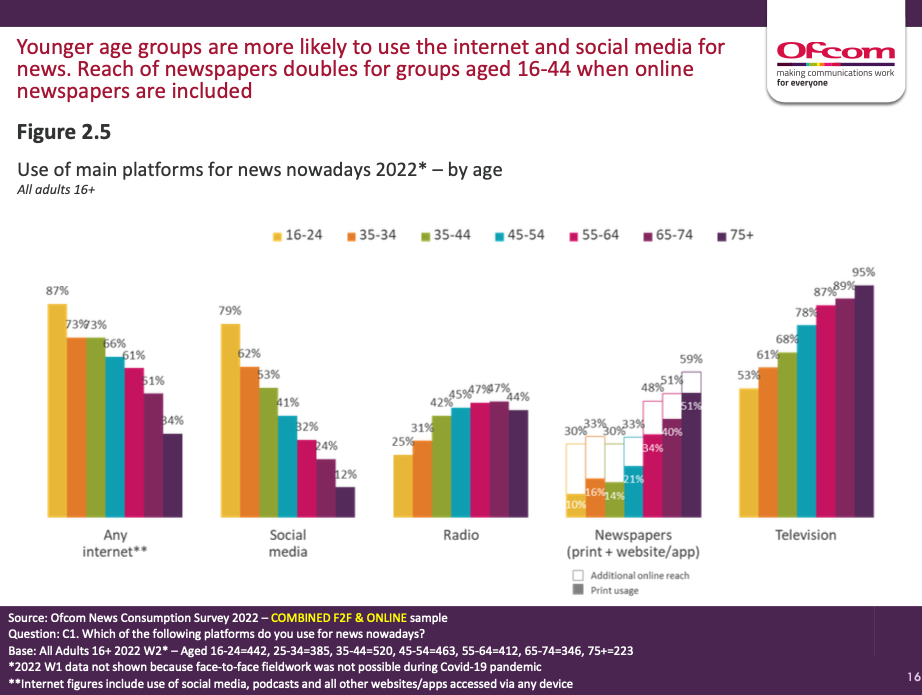
\includegraphics[width=10cm]{News-Consumption-in-the-UK-2022-report-01}
        \label{fig:my_label}
    \end{figure}
\end{frame}

%----------------------------%
\section{Brexit and Online News}

\begin{frame}{Online Media Consumption and Brexit}
    \begin{itemize}
        \item How polarised was online media consumption in the UK during the Brexit referendum campaign?
        \item This is my current area of research. Let me show you some of my findings...

    \end{itemize}
\end{frame}

\begin{frame}{Clicks on Brexit News Online}
    \begin{figure}
        \centering
        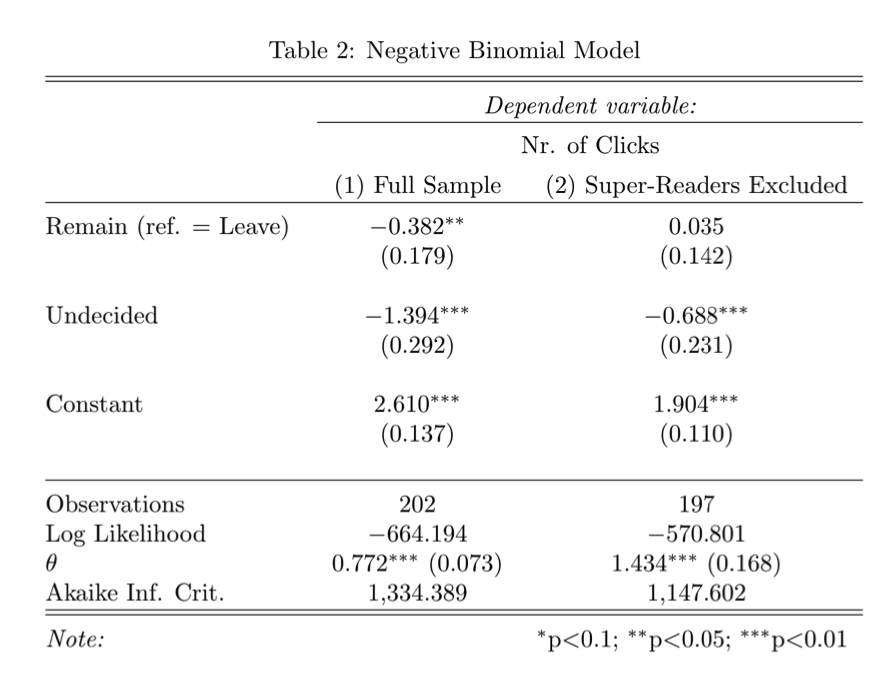
\includegraphics[width=9cm]{Jarnach-ch1-01}
        \caption{Jarnach, forthcoming}
        \label{fig:my_label}
    \end{figure}
\end{frame}

\begin{frame}{Online Audience Network of Brexit News}
\small Jarnach (forthcoming)
    \begin{figure}
        \centering
        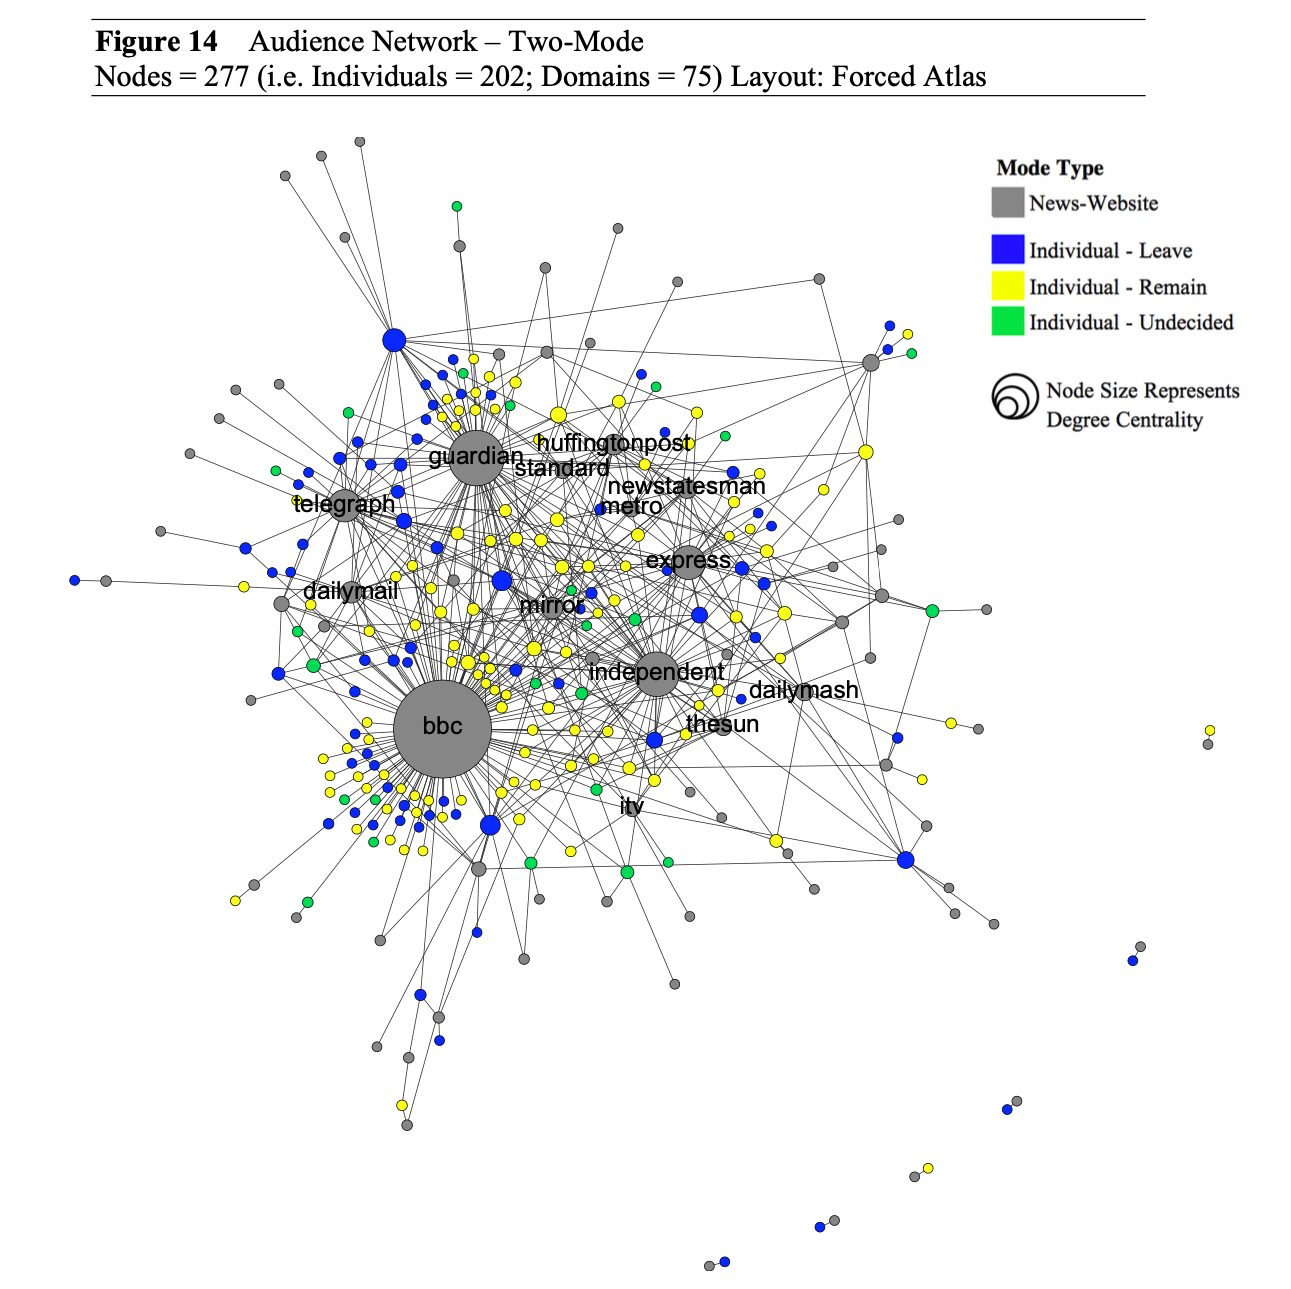
\includegraphics[width=9cm]{Jarnach-ch1-02}
        \caption{Jarnach, forthcoming}
        \label{fig:my_label}
    \end{figure}
\end{frame}

\begin{frame}{Online Audience Network of Brexit News}
\small Jarnach (forthcoming)
    \begin{columns}
        \column{0.5\textwidth}
            \begin{figure}
            \centering
            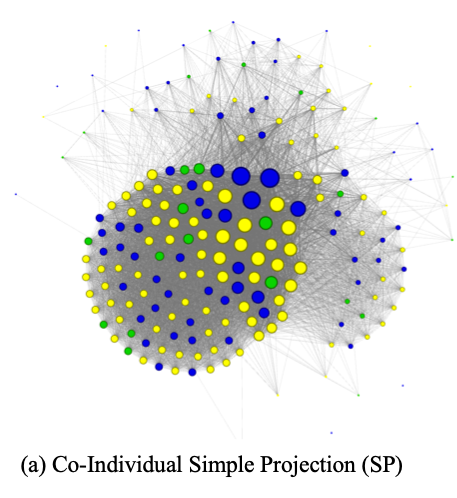
\includegraphics[width=5cm]{Jarnach-ch1-03}
            \end{figure}
   
    \column{0.5\textwidth}
            \begin{figure}
                \centering
                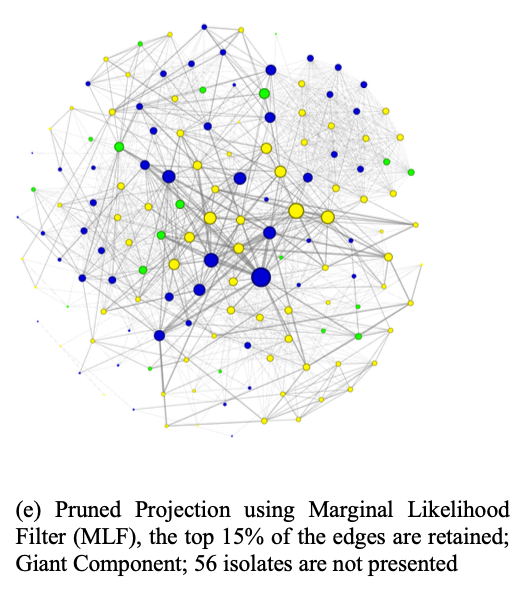
\includegraphics[width=5cm]{Jarnach-ch1-04}
            \end{figure}
     \end{columns}
\end{frame}


\begin{frame}{Consumption of political news is low}
\small Jarnach (forthcoming)
            \begin{figure}
                \centering
                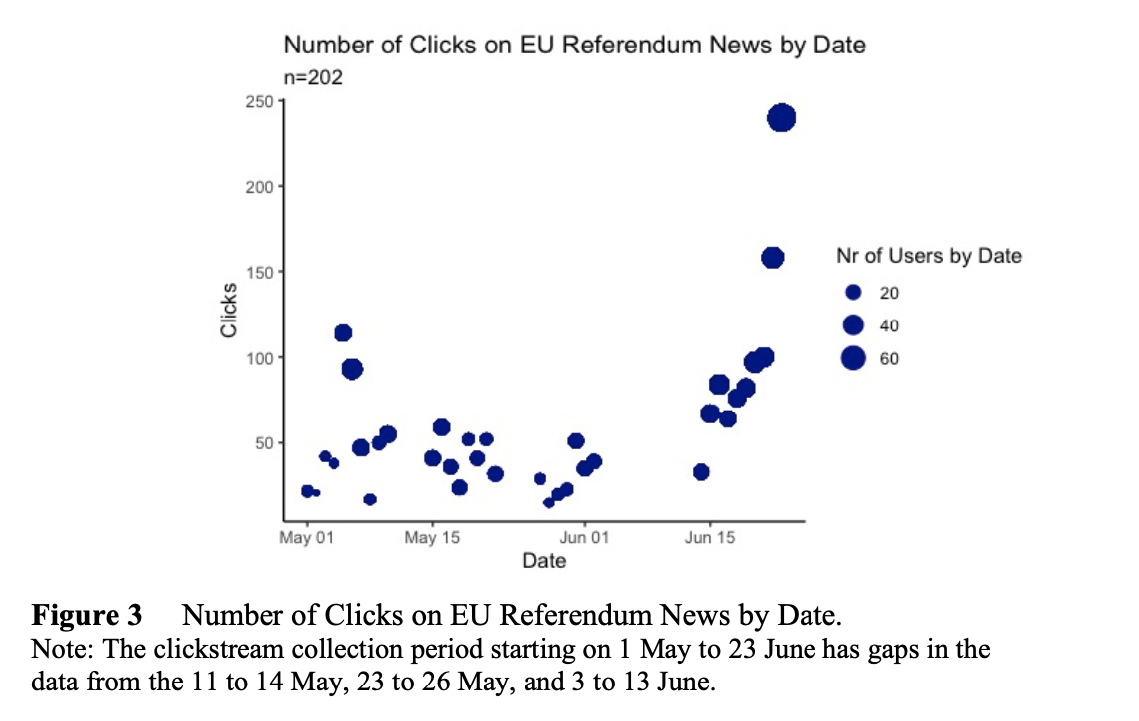
\includegraphics[width=10cm]{Jarnach-ch1-05}
            \end{figure}
\end{frame}




%----------------------------%
\section{Does it matter? }
\begin{frame}{But does it matter? Yes}
\begin{itemize}
    \item Research by Andersen et al. (2002) concludes that political knowledge of the electorate matters, as individuals with higher knowledge are more likely to match their issue preferences to party platforms.
    \item Those generally more interested and engaged in politics are more likely to form an opinion and be internally coherent in their political attitudes and beliefs (e.g. Berelson et al., 1966; Lazarsfeld, et al., 1948; Baldassarri & Gelman, 2008).
\end{itemize}
\end{frame}

\begin{frame}{But does it matter? No}
\begin{itemize}
    \item Rational ignorance (Downs, 1957) refers to a situation where individuals deliberately choose not to acquire certain information or knowledge because the cost of obtaining that information exceeds the potential benefits they would gain from it. 
    \item Political ignorance may not matter because individuals with limited knowledge can still make sound decisions by relying on informational cues (e.g. Page and Shapiro 1992; Wittman 1995; Lupia and McCubbins 1998).
    \item  If voter ignorance is random and unbiased, it might not have a significant impact on election outcomes because uninformed voters' preferences would effectively cancel each other out. (Wittman, 1995)
\end{itemize}
\end{frame}

%----------------------------%
\section{Discussion}
\begin{frame}{Discussion}
\begin{itemize}
    \item Is it irresponsible to let people vote without prior knowledge and training?
    \item Can we ask every citizen to decide on every political decision?
    \item Do citizens have the time,  money, and knowledge to make such decisions?
    \item What decisions should be down to the citizens? which decisions should be made by the “professionals”?
    \item Should some people get more votes than others?
    \item Who should get more votes than others?
    \item Is electing a representative just handing over your votes to that person? how is that different from giving unequal numbers of votes to people?
    \item Is online News bad for Democracy? 
\end{itemize}
\end{frame}



%----------------------------%
% Contact
\begin{frame}
    \frametitle{Contact}
    \centering
    
    \Large\color{oxfordblue}
    Thank you!
    

    \vspace{0.5cm}
        \textit{clemens.jarnach@gtc.ox.ac.uk \\ 
        \href{https://clemensjarnach.github.io}{https://clemensjarnach.github.io}}

\end{frame}
%----------------------------%

% References slide
\begin{frame}
\frametitle{References}
\tiny
\nocite{*}
\bibliographystyle{amsplain}
\bibliography{UVU}

\end{frame}

%%%%%%%%%%%%%%%%%%%%
\end{document}
%%%%%%%%%%%%%%%%%%%%
